\begin{displayquote}
	\textsf{After the validation of the numerical and parallel performance of $m$-UCGLE, a major difficulty to profit from UC methods including $m$-UCGLE is to implement the manager engine which can well handle their fault tolerance, load balance, asynchronous communication of signals, arrays and vectors, the management of different computing units such as GPUs, etc. In Chapter \ref{UCGLE for Linear Systems with Multiple Right-hand-sides}, we tried to give a naive implementation of the engine to support the management computing components on the homogeneous/heterogeneous platforms based on MPI\_SPAWN and MPI non-blocking sending and receiving functionalities. The stability of this implementation of the engine cannot always be guaranteed. Thus we are also thinking about to select the suitable workflow/task based environments to manage all these aspects in the UC approach. YML\footnote{http://yml.prism.uvsq.fr/} is a good candidate, which is a workflow environment to provide the definition of the parallel application independently from the underlying middleware used. The special middleware and workflow scheduler provided by YML allows defining the dependencies of tasks and data on the supercomputers \cite{delannoyyml}. YML, including its interfaces and compiler to various programming languages and libraries, will facilitate the implementation of UC based methods with different numerical components. In this chapter, firstly we give a quick summary of the YML framework, and then analyze the limitations of existing YML implementation for UC approach. In the end, we propose the related solutions.}
\end{displayquote}

\vspace{0.6in}


\section{YML Framework}

YML is a workflow environment dedicated to the execution of parallel de distributed applications on various middleware. The YML framework enables the description of the complex parallel application based on the tasks. The task-based application written based on YML language can be executed on several runtime-systems or middleware without changes. YML is a software layer between the end-user and the runtime system of a supercomputer and/or the middleware of a distributed system, which is in charge of communication. 

\subsection{Structure of YML}

YML is composed of three main parts: an IDL, a kernel and a back-end allowing interactions with the runtime-system or middleware. A high-level workflow language, a just-in-time scheduler and a system of service integration constitute the kernel of YML. The high-level language which is XML-based permits the description of the graph of application. The nodes of the graph correspond to computation while edges correspond to dependencies or communications. A component could be itself a graph. The language integrates the ability to describe components on the one hand and application graphs on the other hand. Both aspects are encapsulated in XML document for homogeneity. This language provides a way to specify the communication between components during the execution of the application. The graph can contain parallel and sequential sections and standard construction of most languages including branching, exceptions, and loops. The graph language describes the dependencies between the components during the execution. These dependencies rest on the notion of events. The compiler translates the graph of components of applications in an internal representation containing a set of components calls. The scheduler manages application execution and acts as a client for the underlying runtime system accurately requiring computing resources. During the application execution, the scheduler detects tasks ready for execution solving dependencies at runtime. Each scheduling step may or may not generate a set of parallel tasks, which are translated in computing requests to runtime system through dedicated backends. A service in YML can be “any kind” of a component such as a library (or some component of), a data repository, or a catalog of binary components. Thanks to the component-oriented design of YML, it is easy to incorporate new ones. The computation components can be written in different programming languages like XMP. In the case of using XMP in YML, the tasks, written in XMP are expected to be executed on sub-clusters or groups of nodes, which are tightly connected. These tasks would be hybrid programs with distributed and shared programming models. The scheduler provided by YML invokes and manages the tasks among the sub-clusters or
groups.

Environments such as YML, allowing the realization of the proposed model must be extensible in all their aspects and offer reusability. Furthermore, the ability thereof to provide dynamic integration of end-users expertise is a significant element.

\subsection{YML Design}

The aim of YML is to provide users with an easy-of-use method to run parallel applications on different Grid platform and supercomputer. The framework can be divided into three parts which are the end-users interface, frontend, and backend. The end-users interface is used to provide an easy-to-use and an intuitive way to submit their applications and applications can be described using a workflow language YvetteML, Frontend is the main part of YML which includes a compiler, scheduler, data repository, abstract and implementation components (shown as Fig. \ref{yml-arch}).

Abstract and implementation components based on function can be reused. The backend is the part to connect different Grid and peer to peer middleware.

The development of a YML application is based on the components approach, and then we will discuss the three kinds of components in detail.

\begin{itemize}
	\item \textbf{Abstract component} defines the communication interface with the other components. This definition gives the name, and the communication channels correspond to a data input, data output or both and are typed. This component is used in the code generation step and to create the graph.
	
	\item \textbf{Implementation component} is the implementation of an abstract component. It provides the description of computations through YvetteML language. The implementation is done by using common languages like C or C++. They can have several implementations for the same abstract component.
	
	\item \textbf{Graph component} carries a graph expressed in YvetteML instead of a description of computation. It provides the parallel and sequential parts of an application and the synchronization events between dependent components. It is a straightforward way for scientific researchers to develop their application.
\end{itemize}

Moreover, those three components are independent of middleware. So, to run an application on another grid environment with a different middleware, the user needs to compile each component for the middleware of his choice. OmniRPC as the backend of YML will be used here.

YML helps the developer in the whole process of parallelizing applications. It starts at the early stage of components creation to the execution of hardly constrained workflow applications on a Grid. Moreover, YML allows the test and validation of those applications on the user computer using a special backend which relies on the multithreading capabilities of the underlying operating system.

YML eases components creation. Existing code can be reused by importing libraries as some new components without any adaptation. Those components are called by the application when computational tasks have to be started. Moreover, the notions of abstract and implementation descriptions of components bring three interesting features for the Grid scheduler that can be included in the framework.

\begin{itemize}
	\item \textbf{data migration} can be easily quantified at the start and at the end of the application thanks to the abstract definition.
	\item \textbf{data used} by a component is clearly defined in the abstract and implementation definitions, therefore this can be used in a checkpointing feature to move a component from a node to an other.
	\item \textbf{computation time} of a component can be evaluated thanks to the implementation definition.
\end{itemize}

The use of Data Repository Servers hides the data migrations to the developer and ensure that necessary data are always available to all components of the application.

\begin{figure}[htbp]
	\centering
	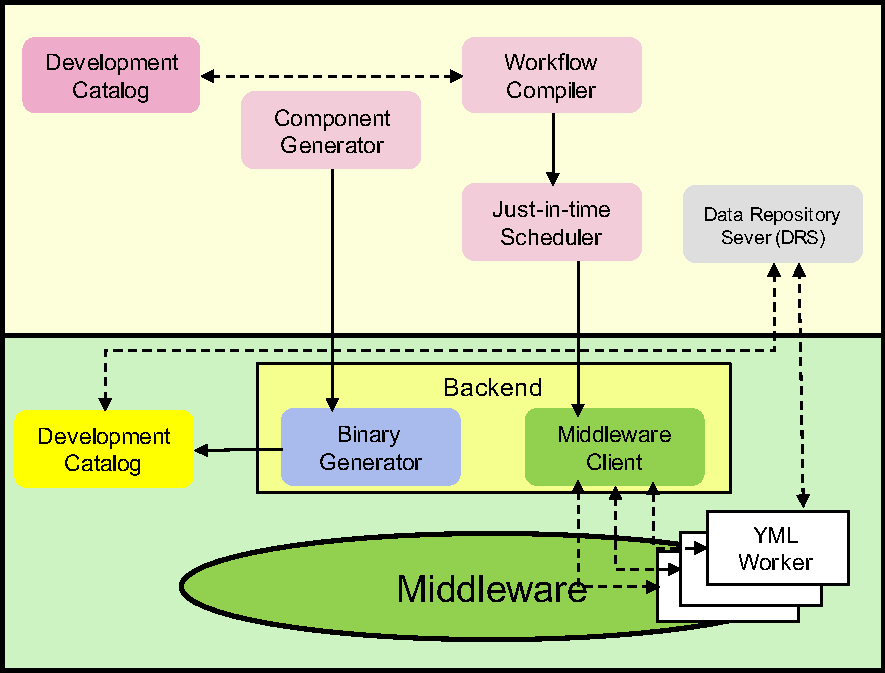
\includegraphics[width=.92\linewidth]{fig/yml-arch.pdf}
	\caption{YML Architecture.}
	\label{yml-arch}
\end{figure}

\subsection{Workflow and Dataflow}

The workflow programming YML faciliates the expression of parallelism for user, which is able to implement the applications in a way very close to the algorithms. Yvette, the high level language provided by YML, is able to describe easily the complex workflow of applications. The \textit{Abstract} provides the interface of components including the input and output data. When a graph of tasks is constructed, the dataflow can be deduced by the input/output data types defined in the \textit{Abstract} of components. As shown in Fig. \ref{fig:yml-dataflow}, YML enables the optimization combining two aspects:

\begin{itemize}
	\item workflow;
	\item dataflow
\end{itemize}

\begin{figure}[htbp]
	\centering
	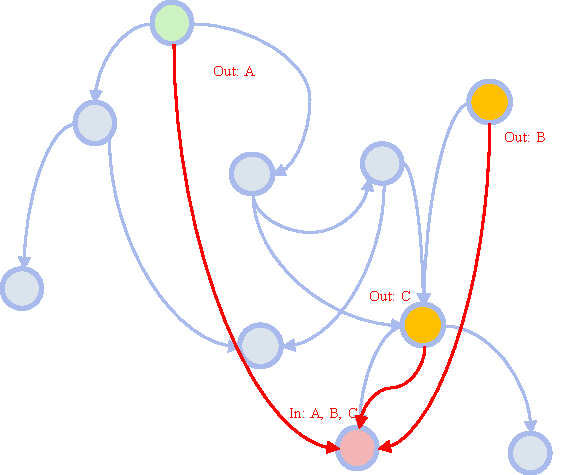
\includegraphics[width=.72\linewidth]{fig/dataflow.pdf}
	\caption{YML workflow and dataflow.}
	\label{fig:yml-dataflow}
\end{figure}

\subsection{Yvette Language}

The YvetteML language provides different features for creating applications. These features are described as below:

\begin{itemize}
	\item \textbf{Parallel Section:} they are used to explicitly define sections which will be executed in parallel. The formule of this operation is given as: \textit{par section 1 // ... // section N endpar};
	\item \textbf{Sequential loop:} they are loops with iterators, which are executed sequentially. The formule of this operation is given as: \textit{seq (i:=begin;end) do ... enddo};
	\item \textbf{Parallel loop:} they are loops with iterators, which are executed in parallel. The formule of this operation is given as: \textit{par (i:=begin;end) do ... enddo};
	\item \textbf{Conditional structure:} they are the condition structure to control the execution of tasks by the condition. The formule of this operation is given as: \textit{if (condition) then ... else ... endif};
	\item \textbf{Synchronization:} The formule of this operation is given as: \textit{wait(event) / notify(event)};
	\item \textbf{Component calls:} the role of component calls is to submit a new task to the Local Ressource Manger providing the name of the component defined earlier and the different input parameters. The formule of this operation is given as: \textit{compute NameOfComponent(args,...,...)}.
\end{itemize}

In the next section, we will give a basic example of YML.

\subsection{YML Example}

In this section, we give an example to understand the grammar and implementation of YML. The workflow of this example is given as Fig. \ref{fig:sum_workflow}. Its scenario is: firstly two seperate sum operations of four given floating numbers are executed, which result in two different floating numbers, these two numbers are added together to output the final results. The exact implementations of this example is given in this section.
 
\begin{figure*}[htbp]
	\centering
	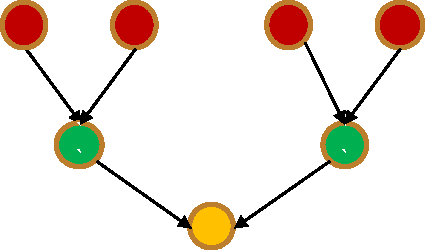
\includegraphics[width=3.in]{fig/sum_workflow.pdf}
	\caption{Workflow of Sum Application.}
	\label{fig:sum_workflow}
\end{figure*}

\subsubsection{Abstract}

The \textit{Abstract} defines the communication interface with the other components. This definition gives the name, and the communication channels correspond to a data input, data output or both and are typed. This component is used in the code generation step and to create the graph. As shown in the code below, the \textit{sum} operation requires two input paramters $a$ and $b$, and an output parameter $res$. These three parameters are all of types \textit{real}. 

\lstset{language=XML}
\begin{lstlisting}[frame=single]
<?xml version="1.0" encoding="utf-8"?>
<component type="abstract" name="test_abstract"
           description="sum of two doubles">
    <param type="real" mode="out" name="res" />
    <param type="real" mode="in" name="a" />
    <param type="real" mode="in" name="b" />
</component>
\end{lstlisting}

\subsubsection{Implementation}

The \textit{Implementation} is the implementation of an abstract component. It provides the description of computations through YvetteML language. The implementation is done by using common languages like C, C++ or XMP. As shown by the code below,  this \textit{sum} operation is implemented to sum the input parameters $a$ and $b$ into the output parameter $res$.

\lstset{language=XML}
\begin{lstlisting}[frame=single]
<?xml version="1.0" encoding="utf-8"?>
<component type="impl" name="test_impl"
          description="sum of two doubles">
    <impl lang="CXX" libs="">
        <header><![CDATA[
          #include <stdlib.h>
        ]]>
        </header>
        <source lang="CXX" libs="">
          res = a + b;
        </source>
        <footer></footer>
    </impl>
</component>
\end{lstlisting}

\subsubsection{Application}

The \textit{Application} carries a graph expressed in YvetteML. It provides the parallel and sequential parts of an application and the synchronization events between dependent components. The code below describes the workflow given in Fig. \ref{fig:sum_workflow}, the two first \textit{sum} operations are executed in parallel, and the output of these operations \textit{res[0]} and \textit{res[1]} are added together by the subsequent sum operation, which gives the final output value \textit{result}.

\lstset{language=XML}
\begin{lstlisting}[frame=single]
<?xml version="1.0" encoding="utf-8"?>
<application name="test_app">
    <description>
        sum application
    </description>
    <params></params>
    <graph>
       nb:=2;
       par (i:=0; nb-1)
       do
           compute test(res[i], 1.0, 2.0); #res[0 or 1]= 3.0
       enddo
       endpar
       compute test(result, res[0], res[1]); #result = 6.0
    </graph>
</application>
\end{lstlisting}

\subsection{Multi-level Programming Paradigm: YML/XMP}

The multi-level programming paradigm YML/XMP is supported by the OmniRPC-MPI Middleware. OmniRPC is a thread-safe remote procedure call (RPC) system, based on Ninf, for cluster and grid environment. It supports typical master/worker grid applications. Workers are listed in a XML file named as the host file. For each host, the maximum number of job, the path of OmniRPC, the connecion protocol (ssh, rsh) and the user can be defined.

An OmniRPC application contains a client program which calls remote procedures through the OmniRPC agent. Remote librairies which contain the remote procedures are executed by the remote computation hosts, there are implemented like a executable program which contains a network stub routine as its main routine. The declaration of a remote function of remote library is defined by an interface in the Ninf interface definition language (IDL). The implementation can be written in familiar scientific computation language like FORTRAN, C or C++.

There are two versions of OmniRPC, one is for grid computation and the other for supercomputer. The first one (the original version) was designed for the grid computing and distributed architecture of large numbers of computers. The second one was created specially for supercomputers, the XMP language is only usable with this version of OmniRPC if we want to use YML in complement.

The multilevel programming model with the combination of YML and XMP can be described as:

\begin{itemize}
	\item High level: communication inter nodes/group of nodes
	\begin{itemize}
		\item YML - coarse grain parallelism - asynchronous communication
	\end{itemize}
	\item: Low level: group of nodes / cores
	\begin{itemize}
			\item PGAS language XMP programming with pragma
		\end{itemize}
\end{itemize}

\begin{figure}[t]
	\centering
	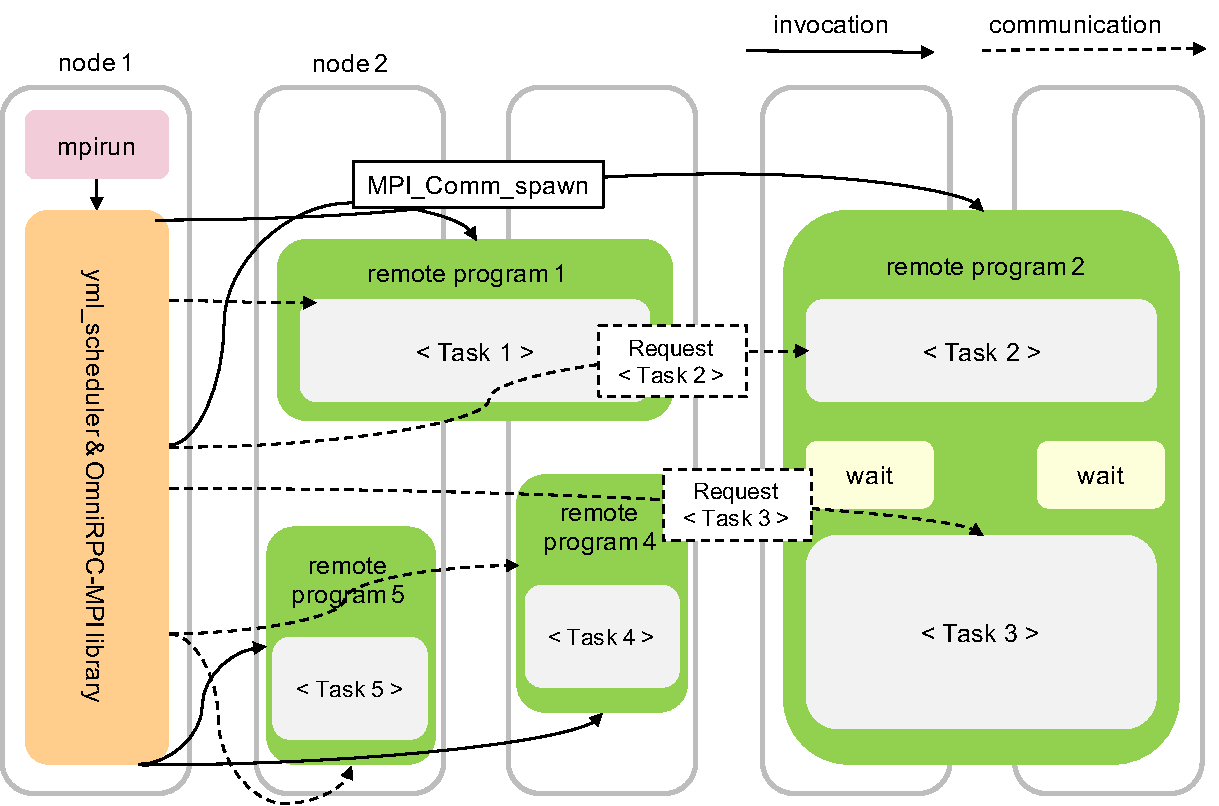
\includegraphics[width=.92\linewidth]{fig/xmp-yml-exec.pdf}
	\caption{Application Execution with YML + OmniRPC-MPI.}
	\label{xmp-yml-exec}
\end{figure}


\section{Limitations of YML for UC Approach}\label{Limitations of YML for UC Approach}

In this section, we analyze the limitations of YML for the implementation of UC approach.

\subsection{Workflow of $m$-UCGLE Analysis}

In order to analyze the possibility to implement unite and conquer methods by YML framework, in this section, we give the workflow of $m$-UCGLE as Fig. \ref{m-UCGLE-task}. When the application starts, various number of components/tasks are allocated (e.g. three GMRES, 2 ERAM and 1 LSP components in the Fig. \ref{m-UCGLE-task}). The first state for GMRES and ERAM components is the \textit{Initialization} (denoted as I in the figure) which loads the matrix and vectors. Then the Arnoldi reduction processes are executed for them (denoted as A in the figure); for GMRES, a temporary solution can be approached by solving a least squares problem (denoted as L in the figure), for ERAM, a number of eigenvalues can be approximated (denoted as E in the figure); these eigenvalues are asynchronously sent to LP component and generate the LS polynomial preconditioning parameters; these parameters are asynchronously sent to GMRES components and perform the iterative steps to generate a new preconditioned residual vector (denoted as P in the figure), and then restart GMRES; if no parameters recevied from LP component, GMRES are restarted with the residual vector gotten from L. The restarting loop can be stopped, if the stop conditions of all GMRES components are satisfied.

\begin{figure}[t]
	\centering
	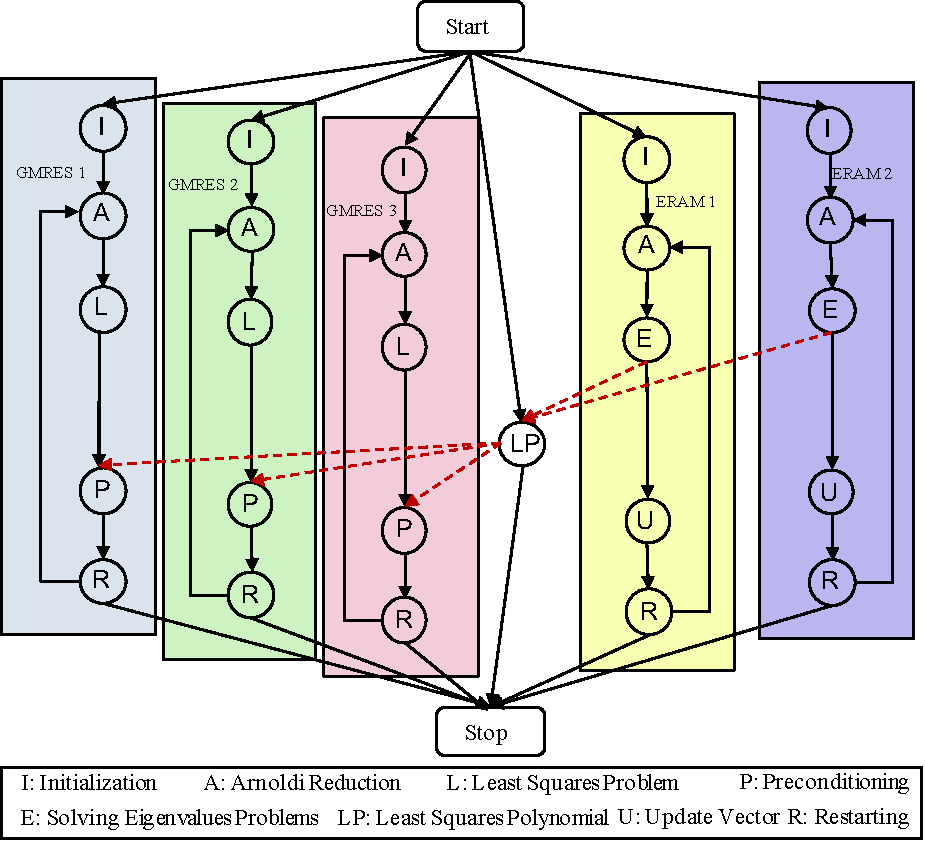
\includegraphics[width=6.2in]{fig/m-UCGLE-task2.pdf}
	\caption{m-UCGLE task.}
	\label{m-UCGLE-task}
\end{figure}

\subsection{Asynchronous Communications}

The first limitation of YML framework for unite and conquer approach is that it does not support the special asynchronous communications (shown as the red dashed arrows in Fig. \ref{m-UCGLE-task}) which send and receive the eigenvalues and preconditioning parameters between different computing components. In details, this type of operations can be summarized as: 1) check the receiving of data asynchronously from other components; 2) if received, perform an operation with these data; if not, perform another operation without these data.

\subsection{Mechanism for Convergence}

The second limitation of YML framework for unite and conquer approach is the lack of a mechanism to check the convergence of iterative methods. In details, for the GMRES components in Fig. \ref{m-UCGLE-task}, they all perform the loop of Arnoldi reduction until the convergence criteria is satisfied or they exceeded the maximum number of iterations allowed. YML does not allows the mechasim to break the loop in halfway with some given condition. The iterative methods can only be implemented with fixed number of iterative steps. This kind of implementations is inefficient for the iterative methods, and the convergence cannot always be guaranteed.

\section{Proposition of Solutions}

We reviewed the grammar and implementation of YML framework, and propose the solution of its limitations for unite and conquer approach discussed in Section \ref{Limitations of YML for UC Approach}.

\subsection{Dynamic Graph Grammar in YML}

The special asynchronous communications of unite and conquer can be expressed with extending YML grammar to support the dynamic graphs.

\subsubsection{Definition of Dynamic Graph}

The dynamic graphs are the types of graph modifiable depends the variables and/conditions. The dynamic graph can be supported with the introduction of a new variable for the dynamic graph in the \textit{Abstract} components:

\lstset{language=XML}
\begin{lstlisting}[frame=single]
<param type="var_graph" mode="inout" name="foo">
\end{lstlisting}

The variable for the dynamic graph can be the mode of \textit{in}, \textit{out} or \textit{inout}. These parameter may be evaluated and modified inside a task, or only as logical into Yvette “if (logical) then $\cdots$ else $\cdots$"; If the computation to evaluate the logical is to complex, we may use a task with a special indication, added on the Implementation component, such as “graph\_scheduler\_evaluation”: then the scheduler may manage those tasks as others, of run it “itself”.

\subsubsection{Scenario Example}

In this section, we give a example for dynamic graphs in YML framework, as shown in Fig. \ref{fig:sum_workflow2}. In details, the red and purple are the addition operations, and the yellow point is the operation to set value. The red dashed arrow signficates an asynchronous depency of data. The priority of setting value in the yellow point is: 1) check the output value $a$ of red point, if this value is odd, then set the value to be $a$; 2) if $a$ is even, set the value to be $b$. This operation is a similar scenario for the asynchronously sending and receiving data in the unite and conquer methods.

\begin{figure*}[htbp]
	\centering
	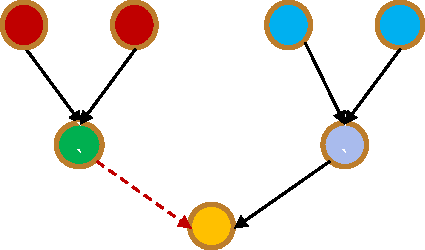
\includegraphics[width=3.in]{fig/sum_workflow2.pdf}
	\caption{New Scenario with Dynamic Graph.}
	\label{fig:sum_workflow2}
\end{figure*}

\textbf{Abstract:} two types of \textit{Abstract} components are constructed as the codes below. 

\vspace{0.2in}
\lstset{language=XML}
\begin{lstlisting}[frame=single]
<?xml version="1.0" encoding="utf-8"?>
<component type="abstract" name="dyntest_abstract"
          description="sum of two doubles #2">
    <param type="real" mode="out" name="val" />
    <param type="real" mode="in" name="a" />
    <param type="real" mode="in" name="b" />
    <param type="var_graph" mode="out" name="odd" /> 
</component>
\end{lstlisting}

\vspace{0.2in}

\lstset{language=XML}
\begin{lstlisting}[frame=single]
<?xml version="1.0" encoding="utf-8"?>
<component type="abstract" name="dyntest_abstract"
          description="set value">
    <param type="real" mode="out" name="val" />
    <param type="real" mode="in" name="a" />
    <param type="var_graph" mode="inout" name="odd" /> 
</component>
\end{lstlisting}

\textbf{Implementation:} two types of \textit{Implementation} components related with the \textit{Abstract} components defined above are constructed as the codes below. 

\vspace{0.2in}
\lstset{language=XML}
\begin{lstlisting}[frame=single]
<?xml version="1.0" encoding="utf-8"?>
<component type="impl" name="dyntest_impl"
          description="sum of two doubles #2">
    <impl lang="CXX" libs="">
        <header><![CDATA[
          #include <stdlib.h>
        ]]>
        </header>
        <source lang="CXX" libs="">
           res = a + b;
           if(res % 2 ==0){
             odd = false;
           } else {
             odd = true;
           }
       </source>
       <footer></footer>
    </impl>
</component>
\end{lstlisting}

\vspace{0.2in}
\lstset{language=XML}
\begin{lstlisting}[frame=single]
<?xml version="1.0" encoding="utf-8"?>
<component type="impl" name="setvalue_impl"
          description="set value">
    <impl lang="CXX" libs="">
        <header><![CDATA[
          #include <stdlib.h>
        ]]>
        </header>
        <source lang="CXX" libs="">
          val = a;
        </source>
        <footer></footer>
    </impl>
</component>
\end{lstlisting}

\textbf{Application:} \textit{Application} component is defined as the below, which describes the workflow of applications.

\vspace{0.2in}
\lstset{language=XML}
\begin{lstlisting}[frame=single]
<?xml version="1.0" encoding="utf-8"?>
<application name="dyntest_app">
    <description>
      set value application
    </description>
    <params></params>
    <graph>
      compute dyntest(res1, 1.0, 2.0, odd); #res = 3.0
      compute test(res2, 4.0, 6.0); #res = 10.0
      if(odd) then
         compute setvalue(val, res1, odd); #val = 3.0
      else
        compute setvalue(val, res2, odd); #val = 10.0
      endif
    </graph>
</application>
\end{lstlisting}


\subsection{Exiting Parallel Branch}

The mechanism for checking the convergence can be etablished by the definition of modes to exit a parallel branch. As shown by Fig. \ref{fig:exit}, there are several types of modes to exit a parallel branch:

\begin{enumerate}
	\item the application may exit the parallel branch if all the running tasks are completed;
	\item the application may exit the parallel branch if only several tasks among all are completed;
	\item for the application with multi-level parallelism, we may decide to exit several levels of parallelism;
	\item we may stop completely the computation without any condition.
\end{enumerate}


\begin{figure*}[t]
	\centering
	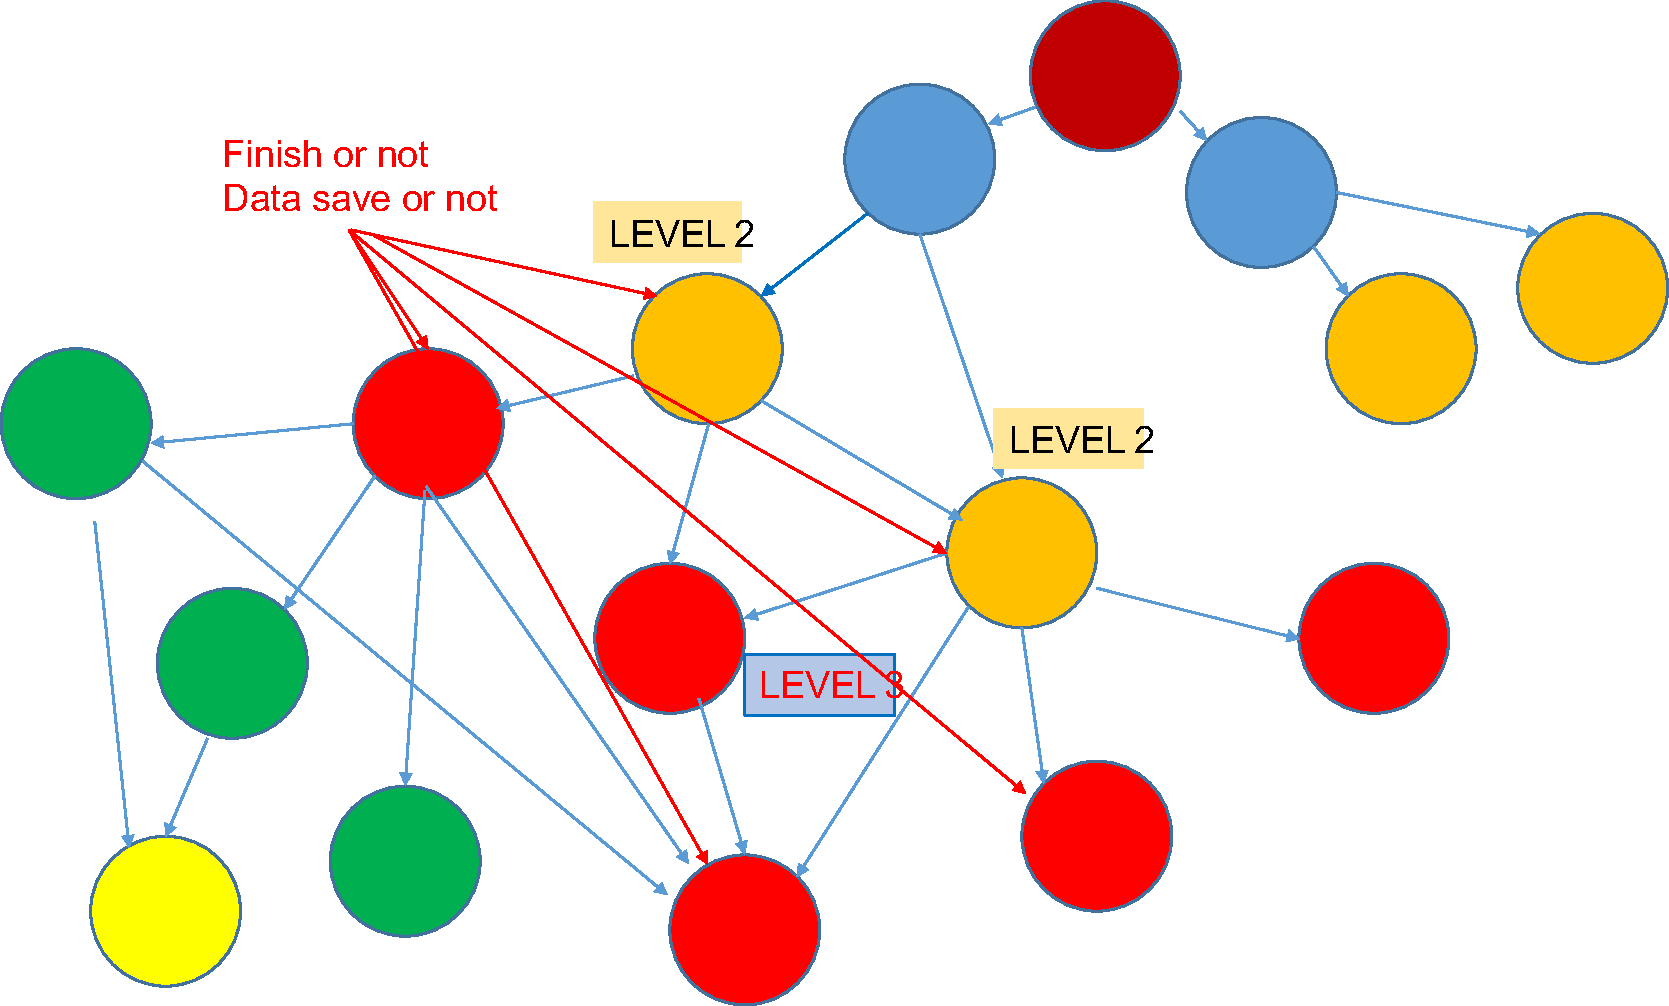
\includegraphics[width=5.in]{fig/exit-branch.pdf}
	\caption{Exiting Parallel Branch.}
	\label{fig:exit}
\end{figure*}

A \textit{Exit} feature for Yvette should be implemented to support the different modes of exiting a parallel branch:

\begin{enumerate}
	\item \textit{Exit(level=p)}: we exit $p$ levels of parallelism ($p$ loops if it is parallel loops);
	\item \textit{Exit(complete=all)}: all the running tasks of the level are finished before to exit;
	\item \textit{Exit(level=p,auto)}: we add to each abstract components if the task has to be finished, data saved or not, we exit the parallel branch ( </exit finish = “yes” />  ) ; 
	and we may ask in the asbtract component:
	
	\lstset{language=XML}
	\begin{lstlisting}[frame=single]
<param type="real" mode="inout" name="A" save_exit="yes"/>
	\end{lstlisting}
	
\end{enumerate}


\subsection{Check Pointing}

\lstset{language=XML}
\begin{lstlisting}[frame=single]
<?xml version="1.0" encoding="utf-8"?>
<application name="dyntest_app">
<description>
check-pointing example
</description>
<params></params>
<graph>
    par:
    	.../...
    	par (i:=0,8) do
    		.../...
    			par 
    				//
    				wait (event1); 
    				if(foo) then 
    					check (level=1);
    				endif
    				//
    			endpar
    		check(i:=2:4)
    		//
    	enddo
    	endpar
    	//
    endpar
</graph>
</application>
\end{lstlisting}


\subsection{$m$-UCGLE Implementation by YML}

\lstset{language=XML}
\begin{lstlisting}[frame=single]
<?xml version="1.0" encoding="utf-8"?>
<application name="dyntest_app">
<description>
m-UCGLE prototype
</description>
<params></params>
<graph>
ngmres: = 3;
neram: = 2;
par
	par(gid: = 0; ngmres-1)
	do
		compute gmres_init(gid, ... );
		compute gmres_ar(gid, ... );
		compute gmres_ls(gid, ..., x);
		if(lsp)
			compute gmres_precond(gid, ..., x);
		endif
		compute gmres_restart(gid, ..., x);
		exit(auto);
	enddo
	
	par(eid: = ngmres; ngmres+neram-1)
	do
		compute eram_init(eid, ... );
		compute eram_main(eid, ... , eigen);
	enddo
	
	if(eigen)
		compute lsp_init(ngmres+neram, ... , lsp);
	endif

endpar
</graph>
</application>
\end{lstlisting}


\section{Demand for MPI Correction Mechanism}

MUST\footnote{https://tu-dresden.de/zih/forschung/projekte/must} detects usage errors of the Message Passing Interface (MPI) and reports them to the user. As MPI calls are complex and usage errors common, this functionality is extremely helpful for application developers that want to develop correct MPI applications. This includes errors that already manifest - segmentation faults or incorrect results - as well as many errors that are not visible to the application developer or do not manifest on a certain system or MPI implementation.

To detect errors, MUST intercepts the MPI calls that are issued by the target application and evaluates their arguments. The two main usage scenarios for MUST arise during application development and when porting an existing application to a new system. When a developer adds new MPI communication calls, MUST can detect newly introduced errors, especially also some that may not manifest in an application crash. Further, before porting an application to a new system, MUST can detect violations to the MPI standard that might manifest on the target system. MUST reports errors in a log file that can be investigated once the execution of the target executable finishes.

\section{Conclusion}

\clearemptydoublepage

\clearemptydoublepage